\documentclass[tikz]{standalone}

\usepackage[T1]{fontenc}
\usepackage[english]{babel}

\usepackage{bm, amsmath, mleftright}
\usepackage{graphicx}

\usepackage{tikz}
\usetikzlibrary{trees, calc}

\begin{document}
    \tikzstyle{level 1}=[level distance=3cm, sibling distance=3cm]
    \tikzstyle{level 2}=[level distance=4cm, sibling distance=2cm]
    
    \tikzstyle{signal}=[rounded corners, draw, align=center]
    \tikzstyle{unamed}=[draw, circle]

    \begin{tikzpicture}[grow=south]
        \node (x) {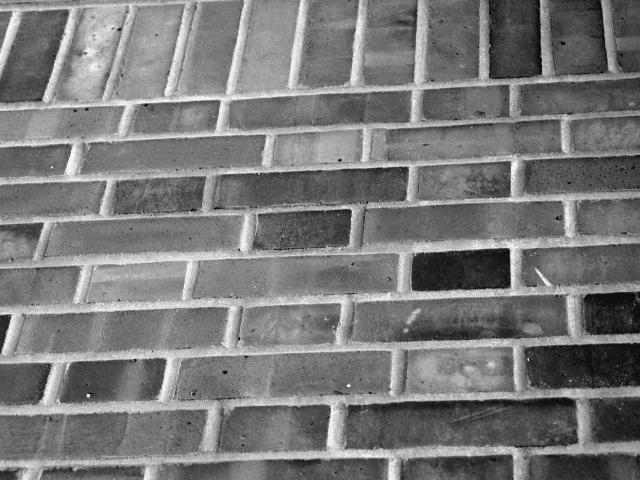
\includegraphics[width=3cm]{images/scatnet/x}}
            child[magenta]{
                node[unamed] (x1_1) {}
                child[magenta]{
                    node[unamed] (x1_1_1) {}
                }
                child[magenta]{
                    node (x1_1_2) {\dots}
                }
                child[magenta]{
                    node[unamed] (x1_1_3) {}
                }
            }
            child[magenta]{
                node (x1_2) {\dots}
            }
            child[magenta]{
                node[unamed] (x1_3) {}
                child[magenta]{
                    node[unamed] (x1_3_1) {}
                }
                child[magenta]{
                    node (x1_3_2) {\dots}
                }
                child[magenta]{
                    node[unamed] (x1_3_3) {} edge from parent node[midway, right, align=center, draw=none] {
                        $\left\lvert \bullet \ostar_{SE(2)} \psi_{i_2, \xi_2, \theta_2}\right\rvert$\\
                        \footnotesize $i_2 = 1, 2, \dots, I$\\
                        $\xi_2= 1, 2, \dots, \lfloor\log_2(L)\rfloor$\\
                        $\theta_2 = 1, 2, \dots, L$
                    }
                } edge from parent node[midway, right, align=center, draw=none] {
                    $\left\lvert \bullet \star \psi_{i_1, \theta_1}\right\rvert$\\
                    \footnotesize $i_1 = 1, 2, \dots, I$\\
                    $\theta_1 = 1, 2, \dots, L$
                }
            };

            \path[draw, blue, ->] (x.200) -- ($(x.200) + (-2, -1)$) node[midway, left] {$\phi_I$} node[signal, anchor=north east] (s0) {\small \(S_0[x]\)};

            \path[draw, blue, ->] (x1_1.200) -- ($(x1_1.south west) + (-1, -.5)$) node[midway, left] {$\phi_I$} node[signal, anchor=north east] {\small \(S_1[x](\bullet, i_1, \theta_1)\)};
            \path[draw, blue, ->] (x1_3.200) -- ($(x1_3.south west) + (-1, -.5)$) node[anchor=north east] (s1_3) {};

            \path[draw, blue, ->] (x1_1_1.200) -- ($(x1_1_1.south west) + (-1, -.5)$) node[midway, left] {$\phi_I$} node[signal, anchor=north east] (s1_1_1) {\small \(S_2[x](\bullet, i_1, \theta_1, i_2, \xi_2, \theta_2)\)};
            \path[draw, blue, ->] (x1_3_1.200) -- ($(x1_3_1.south west) + (-1, -.5)$) node[anchor=north east] (s1_3_1) {};
            \path[draw, blue, ->] (x1_3_3.200) -- ($(x1_3_3.south west) + (-1, -.5)$) node[anchor=north east] (s1_3_3) {};
        \end{tikzpicture}
\end{document}
